\section{Смешанный алгоритм глобального поиска и его эффективная реализация}
Ещё одной модификацией метода Стронгина, позволяющей при оптимизации лучше учитывать данные о локальных оптимумах, найденных в процессе поиска, является смешанный алгоритм Стронгина-Маркина \cite{mixedAlg}.
Наряду с характеристикой интервала \(R(i)\) (\ref{step3_1}) можно рассматривать \(R^*(i)\), которая будет более чувствиетльна к наличию в интревале текущего найденного минимума функции \(x_k^*\):
\begin{displaymath}
R^*(i)=\frac{R(i)}{\sqrt{(z_i-z^*)(z_{i-1}-z^*)}/\mu + 1.5^{-\alpha}}
\end{displaymath}
где \(f(x_k^*)=z^*\), а \(\alpha \in [1;30]\) --- степень локальности. Чем она больше, тем более высокая характеристика у интервала, содержащего \(x_k^*\), по сравнению с остальными.
\par
Смешанный алгоритм состоит в следующем: в процессе работы метода каждые \(S\) итераций интервал для последующего разбиения выбирается по характеристикам \(R^*(i)\). \(S\) --- параметр смешивания.
Такой подход позволяет существенно ускорить сходимость метода. На рис. \ref{fig:localMixOP4d} приведены операционные характеристики чисто глобального и смешанного алгоритма на классе GKLS 4d Simple.
Параметр смешивания \(S\) равен 5, \(\alpha=15\), остальные параметры метода были заданы такие же, как в разделе \ref{sec:multilev_maps}
\begin{figure}[ht]
  \center
  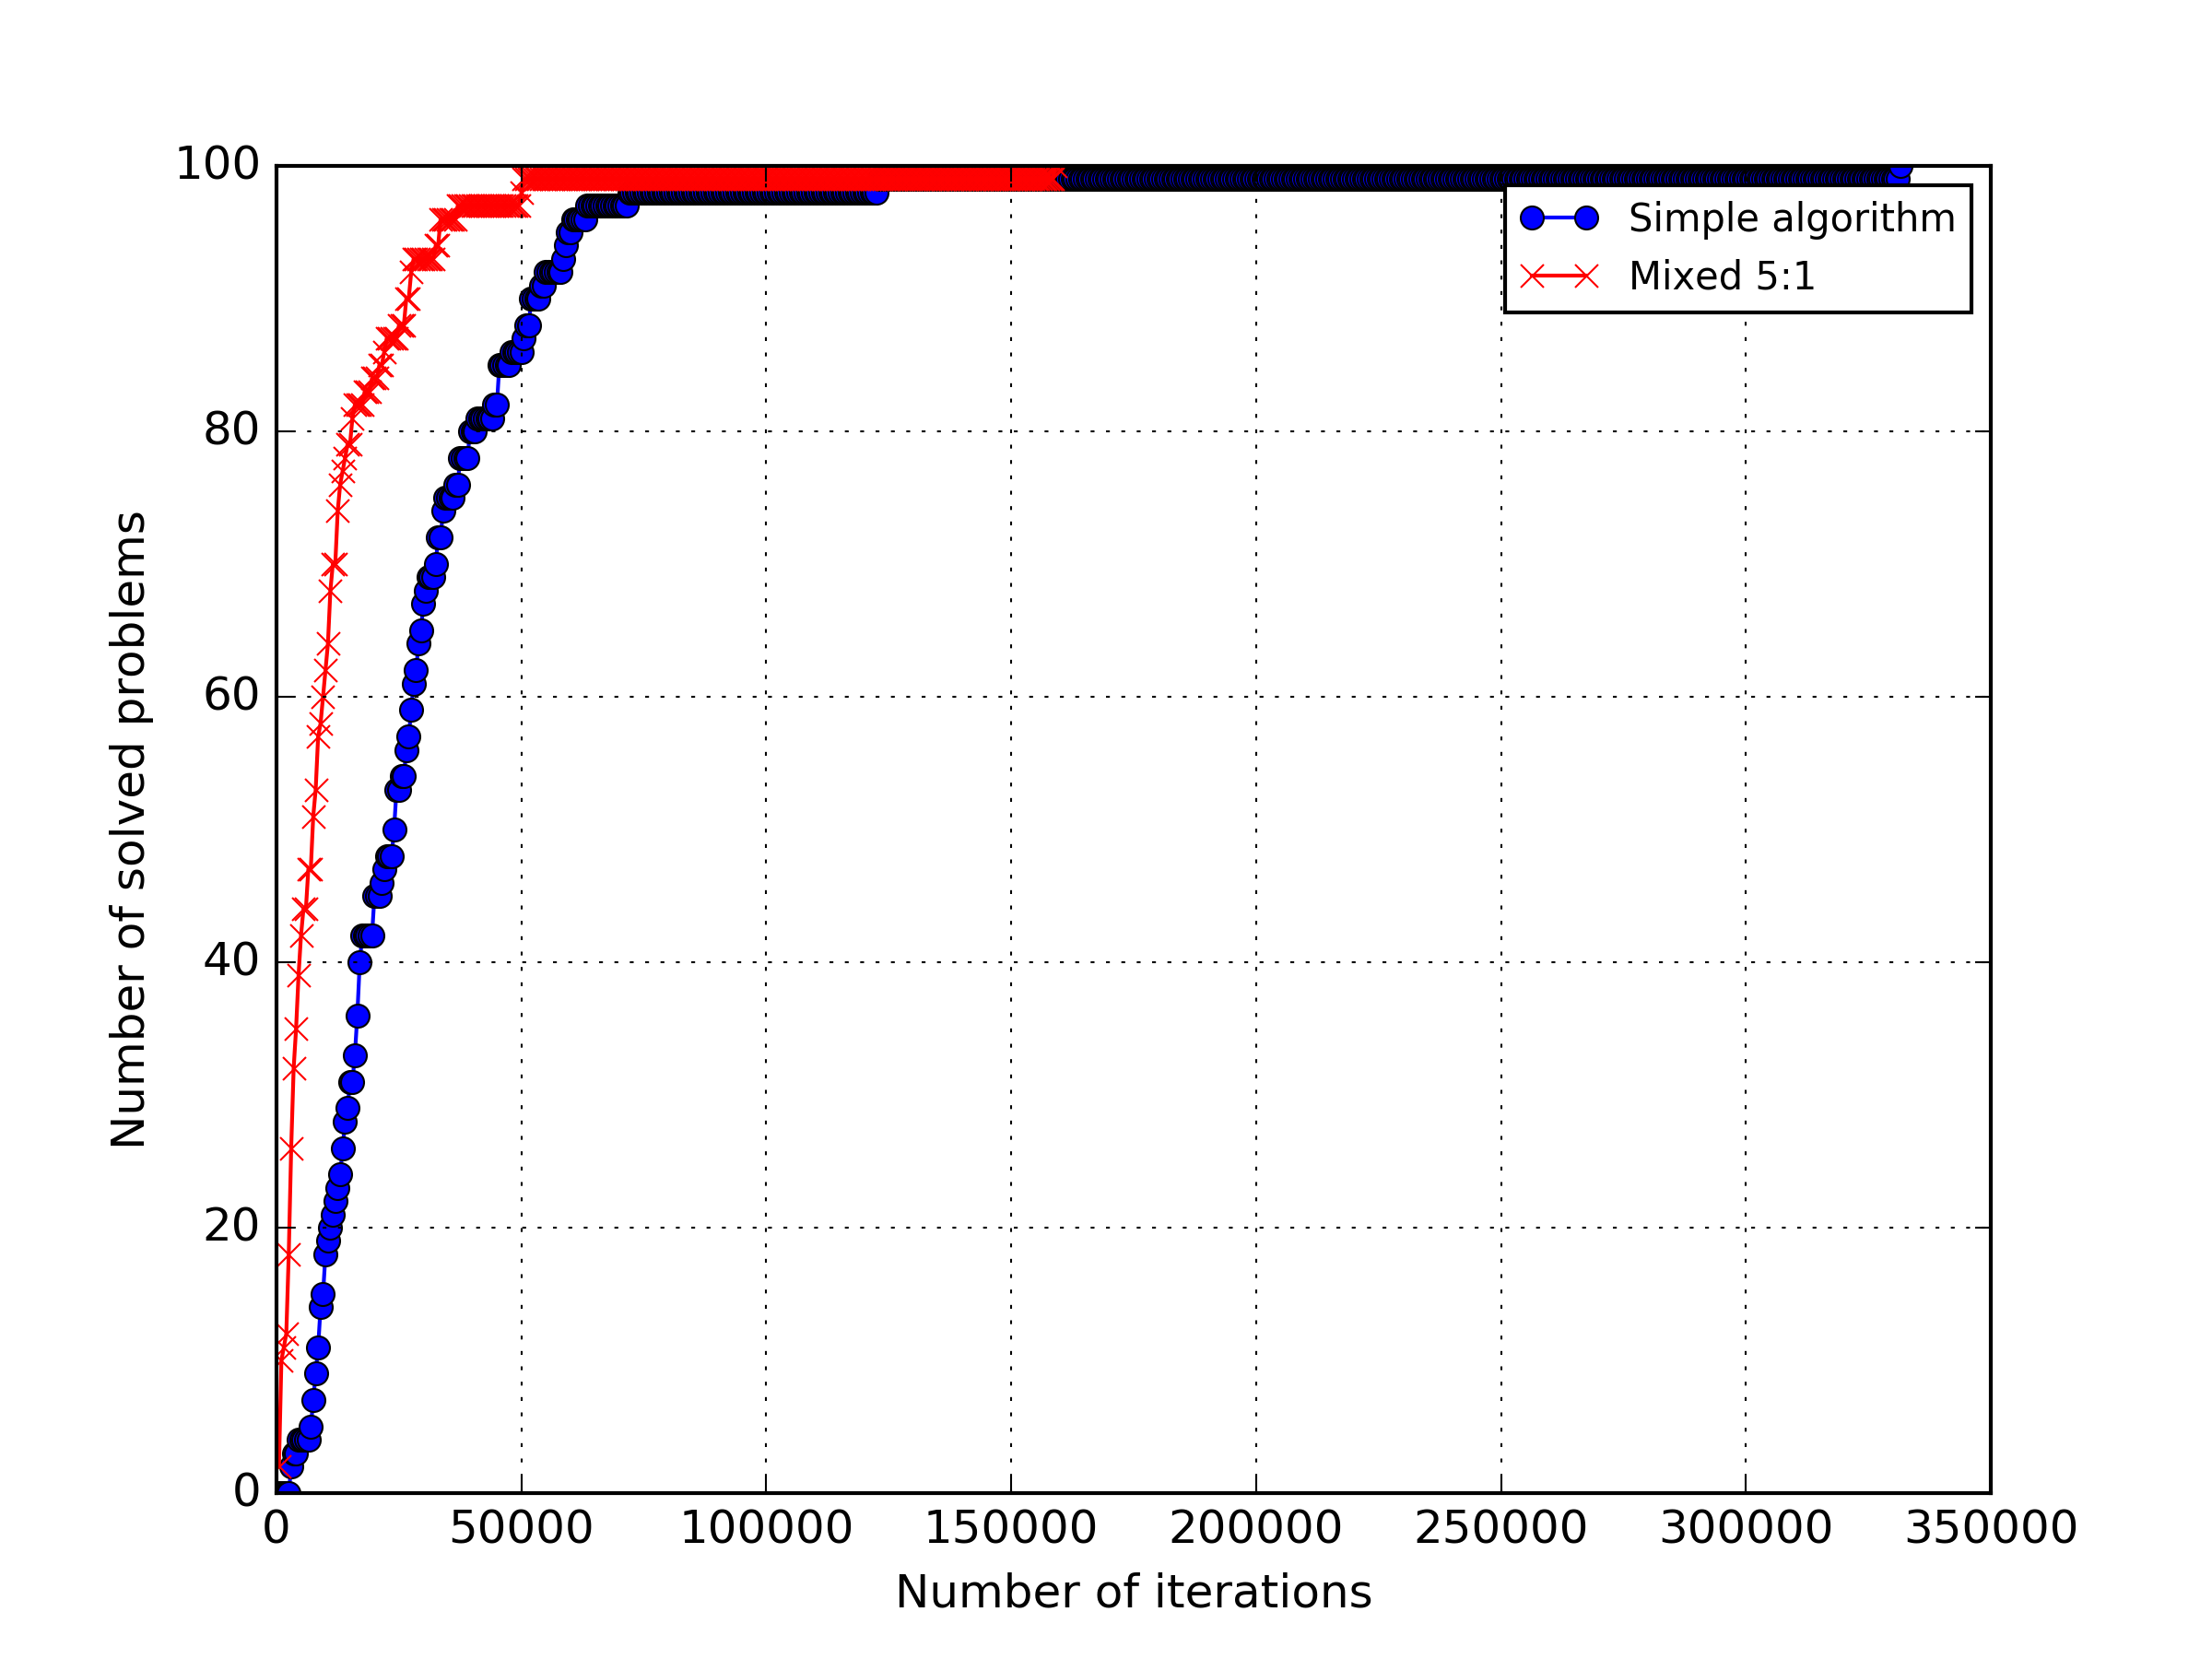
\includegraphics[width=0.75\textwidth]{images/mixed_op4d.png}
  \caption{Операционные характеристики обычного и смешанного АГП на классе GKLS 4d Simple}
  \label{fig:localMixOP4d}
\end{figure}
\par
Из-за того, что интервал имеет сразу две характеристики, появляется проблема эффективной реализации смешанного алгоритма. Если интервал имеет одну характеристику, то для выбора максимальной
достаточно организовать приоритетную очередь характеристик \cite{minmaxheap}.
Причём перезаполнение такой очереди необходимо не на каждой итерации: в большинстве случаев характеристики интервалов не меняются, достаточно удалить разбиваемый интервал и вставить в очередь два новых.
Такая организация работы метода позволяет существенно сократить объём вычислений. При наличии у интервала двух характеристик можно организовать две связанные очереди. В этом случае необходимо предусмотреть
процедуру синхронизации двух очередей.
\par
Перечислим операции, при которых необходима синхронизаия:
\begin{itemize}
  \item вставка интервала сразу в обе очереди;
  \item удаление интервала из какой-либо очереди.
  %\item восстановление внутренней структуры очереди после модификации связанной очереди.
\end{itemize}
\par
Синхронизация достигается путём введения перекрёстных ссылок между элементами очередей. На рис. \ref{fig:heaps} приведена схема связанных очередей. Элемент очереди представляет собой
совокупность ключа (\textbf{LocalR} или \textbf{R}), указателя на интервал (\textbf{pInterval}) и указателя на элемент связанной очереди, соответствующий тому же интервалу (\textbf{pLinkedElement}).
Опишем подробнее алгоритмы вставки и удаления элементов.
\par
Вставка элемента в пару связанных очередей:
\begin{enumerate}
  \item Попытаться вставить элемент в очередь глобальных характеристик (он может быть не вставлен, если имеет слишком низкий приоритет).
  \item Попытаться вставить элемент в очередь локальных характеристик (он может быть не вставлен, если имеет слишком низкий приоритет).
  \item Если элемент интервал вставлен в обе очереди, то выставить перекрёстные ссылки.
\end{enumerate}
\par
Удаление элемента с минимальным ключом:
\begin{enumerate}
  \item Удалить элемент с минимальным ключом из очереди, запомнить указатель \textbf{pLinkedElement}.
  \item Если \textbf{pLinkedElement} ненулевой, то вызвать процедуру удаления элемента, на который указывает \textbf{pLinkedElement} в структуре данных, хранящей связянную очередь.
\end{enumerate}
\par
Последний момент, который надо учесть при реализации: вставка или удаление элемента очереди приводит к тому, что необходимо восстановить её внутреннюю структуру.
Если очередь хранится в куче, то восстанавливается свойство кучеобразности. Во время этого процесса
требуется производить попарные перестановки элементов, а значит, необходимо обновлять ссылки на эти элементы в связанной очереди.
\begin{figure}[ht]
  \center
  \includegraphics[width=0.9\textwidth]{images/examin_heaps.png}
  \caption{Схема устройства связянных очередей}
  \label{fig:heaps}
\end{figure}
\par
Стоит заметить, что внесённые модификации (в основном эта работа со ссылками) не увеличивают ассимптотическую сложность выполнения операций вставки и удаления по сравнению с единственной очередью.
